%
%%%%%%%%%%%%%%%%%%%%%%% file typeinst.tex %%%%%%%%%%%%%%%%%%%%%%%%%
%
% This is the LaTeX source for the instructions to authors using
% the LaTeX document class 'llncs.cls' for contributions to
% the Lecture Notes in Computer Sciences series.
% http://www.springer.com/lncs       Springer Heidelberg 2006/05/04
%
% It may be used as a temlpate for your own input - copy it
% to a new file with a new nam eand use it as the basis
% for your article.
%
% NB: the document class 'llncs' has its own and detailed documentation, see
% ftp://ftp.springer.de/data/pubftp/pub/tex/latex/llncs/latex2e/llncsdoc.pdf
%
%%%%%%%%%%%%%%%%%%%%%%%%%%%%%%%%%%%%%%%%%%%%%%%%%%%%%%%%%%%%%%%%%%%


\documentclass[runningheads,a4paper]{llncs}

\usepackage{amssymb}
\setcounter{tocdepth}{3}
\usepackage{graphicx}
\usepackage{amsmath}
\usepackage{booktabs}
%\usepackage{times}
\usepackage{perpage}
\usepackage{hyperref}
\MakePerPage{footnote}
\usepackage{multirow}
\usepackage{epstopdf} %converting to PDF
\usepackage{tikz}
\usetikzlibrary{arrows,patterns,automata,backgrounds,decorations,fit,petri,positioning,petri,shapes,calc}
\usepackage[caption=false]{subfig}
\usepackage{url}

\urldef{\mailsa}\path|{andriiro,f.m.maggi,marlon.dumas}@ut.ee, kerwin.jorbina@gmail.com|
\urldef{\mailsb}\path|dfmchiara@fbk.eu|
\urldef{\mailsc}\path|{ilya.verenich,m.larosa,simon.raboczi}@qut.edu.au|
\newcommand{\keywords}[1]{\par\addvspace\baselineskip
\noindent\keywordname\enspace\ignorespaces#1}

\begin{document}

\mainmatter  % start of an individual contribution

% first the title is needed
\title{Nirdizati: A Web-based Tool for Predictive Process Monitoring}

% a short form should be given in case it is too long for the running head
\titlerunning{Predictive Business Process Monitoring with LSTM Neural Networks}

% the name(s) of the author(s) follow(s) next
%
% NB: Chinese authors should write their first names(s) in front of
% their surnames. This ensures that the names appear correctly in
% the running heads and the author index.
%
\author{Andrii Rozumnyi\inst{1}  \and Chiara Di Francescomarino\inst{2} \and Chiara Ghidini\inst{2}  \and Fabrizio Maria Maggi\inst{1} \and \\Ilya Verenich\inst{3,1} \and Kerwin Jorbina\inst{1} \and Marcello La Rosa\inst{3} \and \\ Marlon Dumas\inst{1} \and Simon Raboczi\inst{3}\thanks{Author names are in alphabetical order}}

\institute{University of Tartu, Estonia\\
\mailsa
\and FBK IRST, Trento, Italy\\
\mailsb
\and Queensland University of Technology, Australia\\
\mailsc
}

%
% NB: a more complex sample for affiliations and the mapping to the
% corresponding authors can be found in the file "llncs.dem"
% (search for the string "\mainmatter" where a contribution starts).
% "llncs.dem" accompanies the document class "llncs.cls".
%

\toctitle{Predictive Process Monitoring Using LSTM}
\tocauthor{Authors' Instructions}
\maketitle


\begin{abstract}
In this paper, we present a prototype of a predictive process monitoring engine for process workers and operational managers.
The developed solution, named \emph{Nirdizati}, is a configurable full-stack web application that supports users in selecting the preferred prediction method from the list of implemented methods and enables the continuous prediction of various performance indicators at runtime.
The results of the predictions, as well as the real-time summary statistics about the process execution, are presented in a dashboard that offers multiple visualization options.
The target audience of this demonstration includes process mining researchers as well as practitioners interested in exploring the potential of process monitoring.
\keywords{Process Mining, Predictive Process Monitoring, Machine Learning}
\end{abstract}


\section{Introduction} \label{sec:intro}
\emph{Predictive Monitoring}~\cite{PredictiveMonitoring} is an emerging paradigm based on the continuous generation of predictions and recommendations on what activities to perform and what input data values to provide, so that the likelihood of violation of business constraints is minimized. % and violations can be avoided.
In this paradigm, a user specifies a type of prediction or a measure of interest she is interested in. Based on an analysis of execution traces, the idea of predictive monitoring is to continuously provide the user with predictions and estimated values of the measure of interest. Such predictions generally depend both on: (i) the sequence of activities executed in a given case; and (ii) the values of data attributes after each activity execution in a case.

As an example, consider a doctor who needs to choose the most appropriate therapy for a patient. Historical data referring to patients with similar characteristics can be used to predict what therapy will be the most effective one and to advise the doctor accordingly. Meanwhile, in the context of a business process for managing loan applications, the applicant can be advised on the combinations of the loan amount and the length of loan that are the most likely to lead to acceptance of the application, given contextual information about the application and the personal data of the applicant (e.g., age, salary, etc.).

Several approaches have been proposed in the literature to deal with predictive process monitoring tasks.
However, so far, the predictive monitoring approaches have largely remained in the academic domain and 
have not been widely applied in real-time scenarios, in which users require a continuous predictive support. 

In this paper we present Nirdizati, a pioneering open-source Web-based predictive monitoring tool, which is able to fill this gap 
between research and practice, by providing business analysts with a highly configurable instrument for the configuration,  
generation and analysis of different predictive models; and end-users with continuous runtime predictions.

Nirdizati consists of two components: \textit{Nirdizati Training} and \textit{Nirdizati Runtime}. Nirdizati Training takes as input a business process event log and produces one or more prediction models, which can then be deployed in Nirdizati Runtime. Once a model is deployed, Nirdizati Runtime listens to a stream of events related to a business process, and produces a stream of predictions. These predictions are then visualized in a continuously updated Web dashboard.

\section{Nirdizati Training} \label{sec:training}
Nirdizati Training is the component of Nirdizati that allows users to produce predictive models then used by 
Nirdizati Runtime for making predictions on streams of events. It provides several algorithms for generating 
predictive models for different types of predictions and tailored to each specific dataset. 
For example, it is able to build predictive models for predicting remaining time, the next activity to be 
performed, whether a certain outcome will be achieved and even the overall workload per day.
%
To this aim, the training component of Nirdizati relies on two phases: a training and a validation phase. 
In the former, one or more predictive models are built; in the latter, their suitability to the specific 
dataset is evaluated, so as to support the user in selecting the predictive model that ensures the best results.   

Nirdizati Training is composed of a front-end application, which allows users to configure the predictive models
and to evaluate the prediction results, and a back-end application responsible of the actual training and validation.
The back-end application is in turn composed of the four submodules shown in Figure~\ref{fig:RNNexample}.
A Log Manager is in charge of managing the logs. Uploading and retrieving the logs are the basic operations 
of this module. The Encoder is responsible of parsing the logs, labeling them according to the desired type of prediction,
 and preparing the data for the training phase. 
In the Training submodule, the encoded data are split into training and validation set used for evaluation purposes, 
and the predictive model(s) is(are) built from the training data. Finally, the Evaluation submodule
tests the validation data against the model(s) created to get accuracy measures with respect to the groundtruth, 
available from the complete traces in the validation data.
The back-end application comes with a storage module for saving the uploaded logs and the built predictive models.

%First, we have the Front-end application which acts as the interface for the user to
%select settings used for prediction and to analyze the prediction results. The second
%module is the Log Manager which is responsible for managing the logs. Uploading
%and retrieving the logs are the basic operations of this module. The third module is
%the Encoder which retrieves the log from the storage, parses it and prepares the log for
%the training phase in the Predictive Module. In this part, we retrieve the encoded data,
%split it into training and test set for evaluation, and build the predictive model from the
%training data. Finally, using the test data, we test it against the model created to get its
%accuracy. The aggregation of the results are done in the Evaluation Module which is
%tasked to calculate the error of the prediction model created.

%\vspace{-\baselineskip}
\begin{figure}[t]%[H]
	\centering
	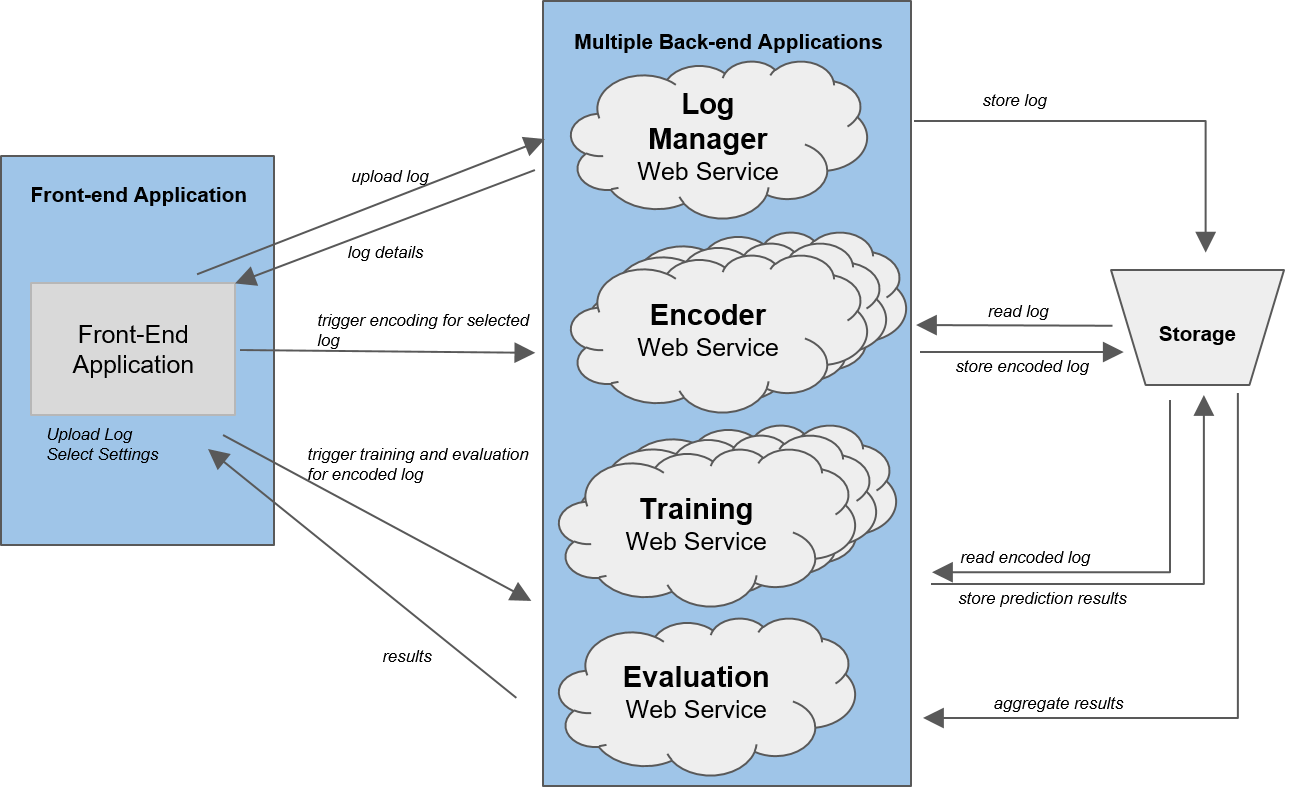
\includegraphics[width=0.7\textwidth]{img/nirdizati-training-architecture-rev}
	\caption{A high-level overview of Nirdizati Training.}
	\label{fig:RNNexample}
\end{figure}
%\vspace{-\baselineskip}

\section{Nirdizati Runtime} \label{sec:runtime}
Figure~\ref{fig:dfd_0} illustrates the flow of data through the proposed system. A workflow management system (WFMS) continuously registers tasks performed in the organization.
This serves as an input to our system, in the form of a stream of events.
Next, the produced stream is consumed by a web server which is responsible for storing data and further information processing. 
Web server, in turn, communicates with a predictive engine which applies pre-trained models for a business process and returns all the results of calculations.
After web server receives the outputs from each predictive model, it writes them to a database and updates corresponding clients.
From the user's side, the results are visualized via a dashboard-based interface which is capable of sending queries requesting various visualization options.

\begin{figure}
	\centering
	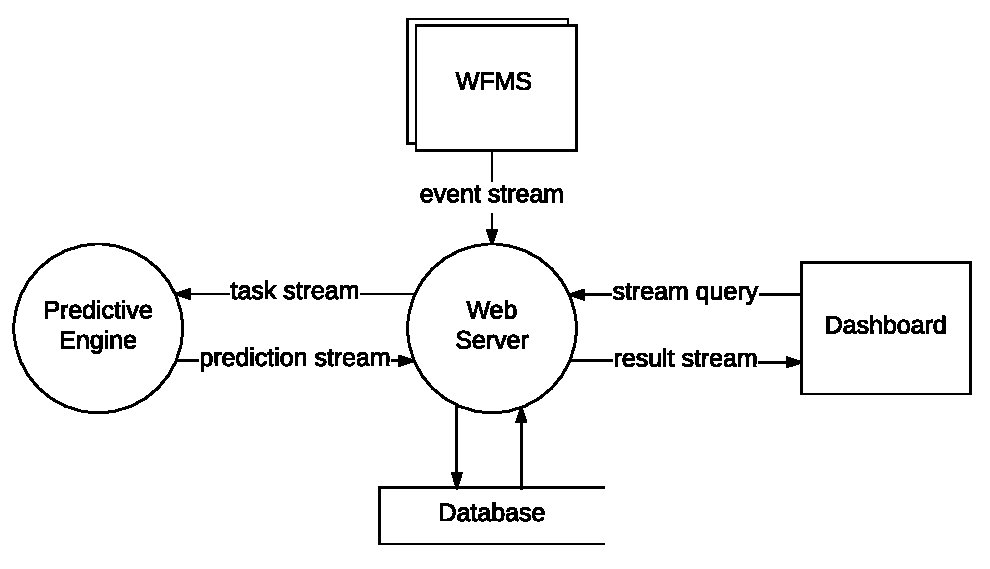
\includegraphics[width=0.7\textwidth]{img/dfd_0}
	\caption{High-level data flow diagram in a Yourdon-Coad notation}
	\label{fig:dfd_0}
\end{figure}

Based on this data flow diagram, we devise the main parts and high-level components of the system (Figure~\ref{fig:arch}): 

\begin{itemize}
	\setlength{\itemsep}{1pt}
	\setlength{\parskip}{0pt}
	\setlength{\parsep}{0pt}
	\item streaming platform
	\item web server with load balancer and internal components
	\item predictive engine
	\item client-side user interfaces
\end{itemize}

\begin{figure}
	\centering
	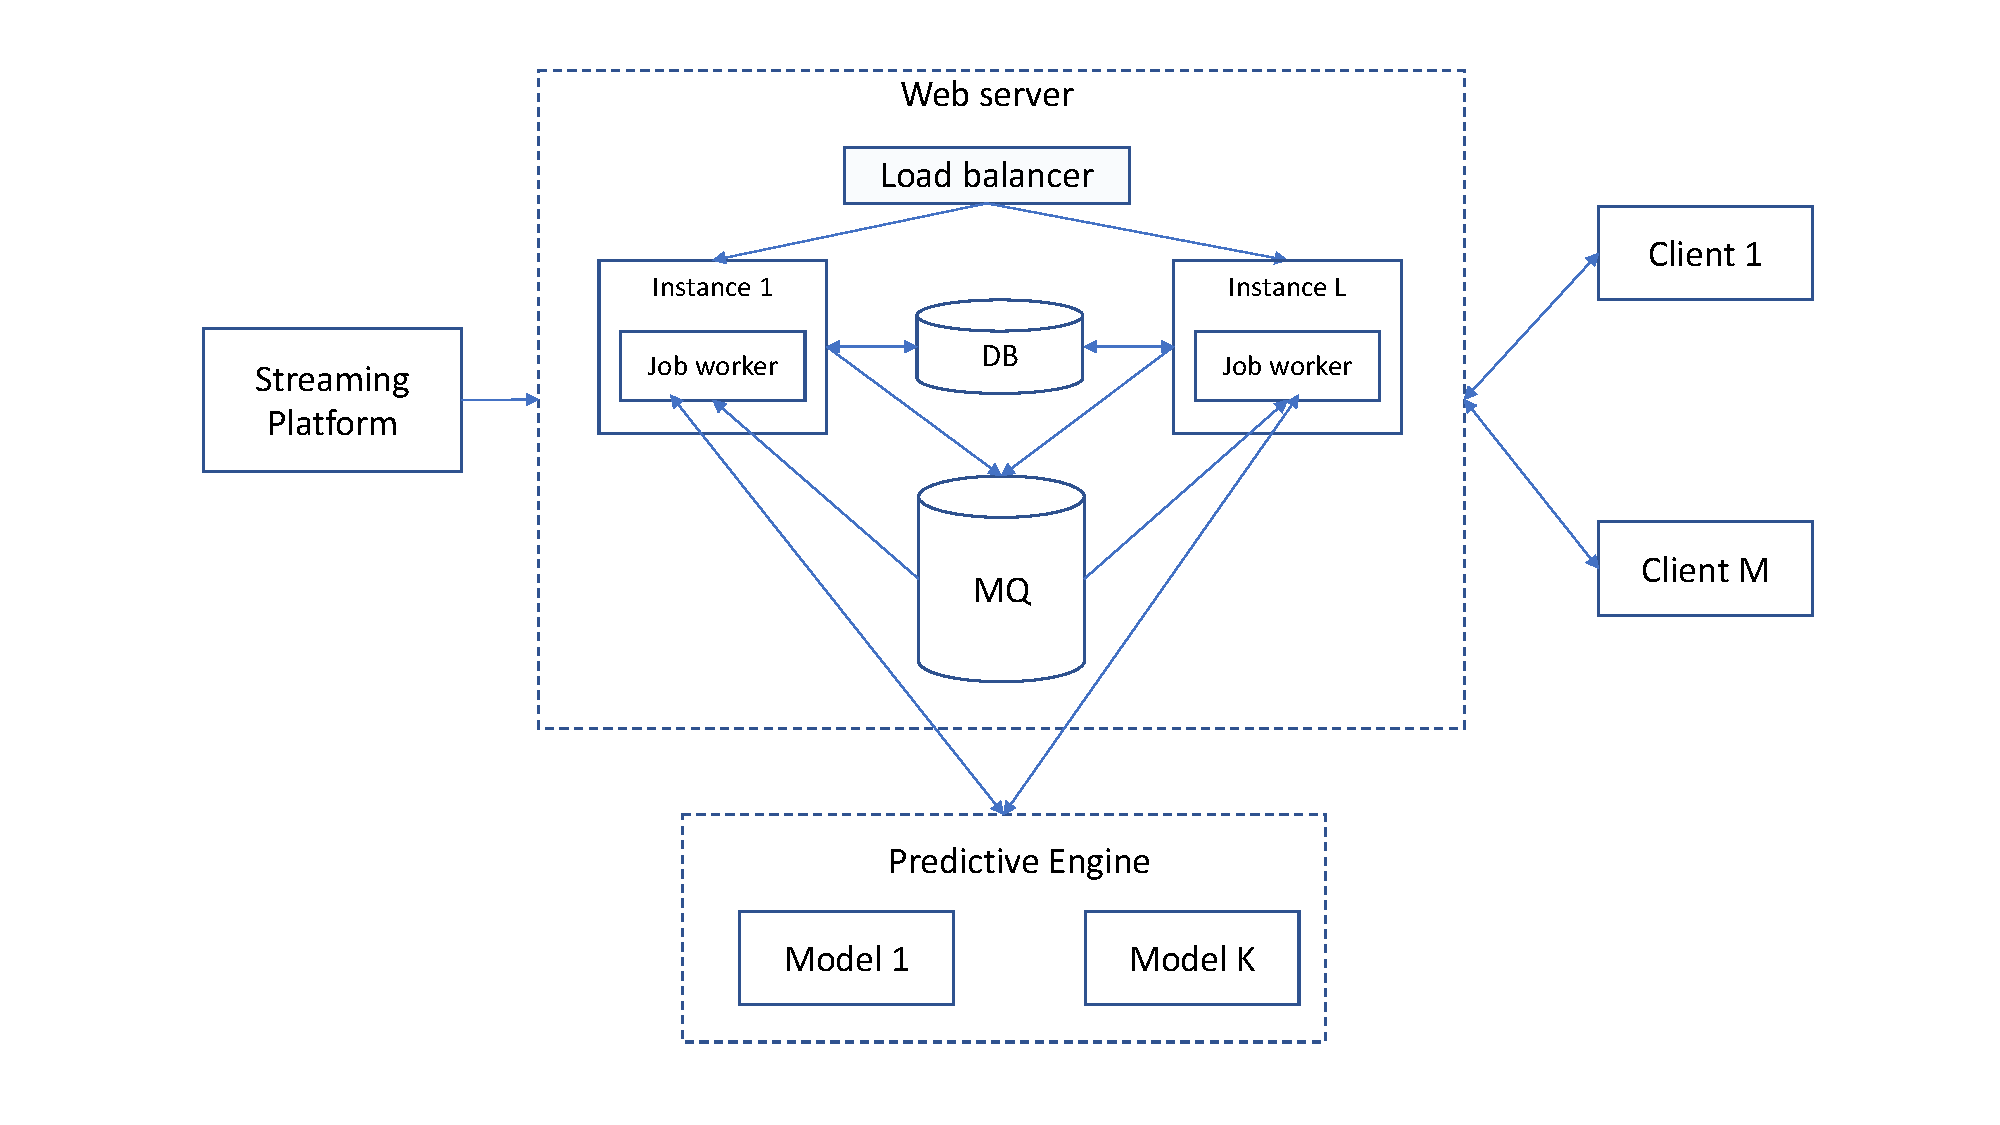
\includegraphics[width=1\textwidth]{img/nirdizati-runtime-architecture}
	\caption{Proposed system design architecture}
	\label{fig:arch}
	%	\vspace{-5\baselineskip}
\end{figure}

Process workers and operational managers – typical users of such system – can set the process performance targets and subscribe to a stream of warnings and alerts generated whenever these targets are predicted to be violated. Thus, process workers will be capable of making more informed, data-driven decisions to get a better control of the process execution. This is especially beneficial for processes where process workers have more leeway to make corrective actions, for example, in a lead management process.

\section{Conclusion} \label{sec:conclusion}
The source code has been released as open source software under the Lesser GNU Public License (L-GPL) at \url{http://github.com/nirdizati}. The developed engine has been deployed on the server belonging to the Institute of Computer Science and can be accessed at \url{http://nirdizati.com}.
\bibliographystyle{splncs03}
\bibliography{paper}

\end{document}
